\section{Modelagem analítica/formal (PRISM) do sistema}

Inicialmente, as constantes de confiabilidade foram inferidos a partir
da experiência com o programa.

Para este documento, no entanto, foi realizado um estudo mais
detalhado destas probabilidades, utilizando os logs de execução do
programa durante os meses de agosto a setembro. As falhas e erros
durante este período de execução, bem como o tempo em que ele
ficou indisponível devido a algum dos componentes foram usados para
chegar aos resultados finais, que podem ser conferidos no modelo
PRISM em~\ref{sec:prism}.

\begin{figure}[htbp]
\centering
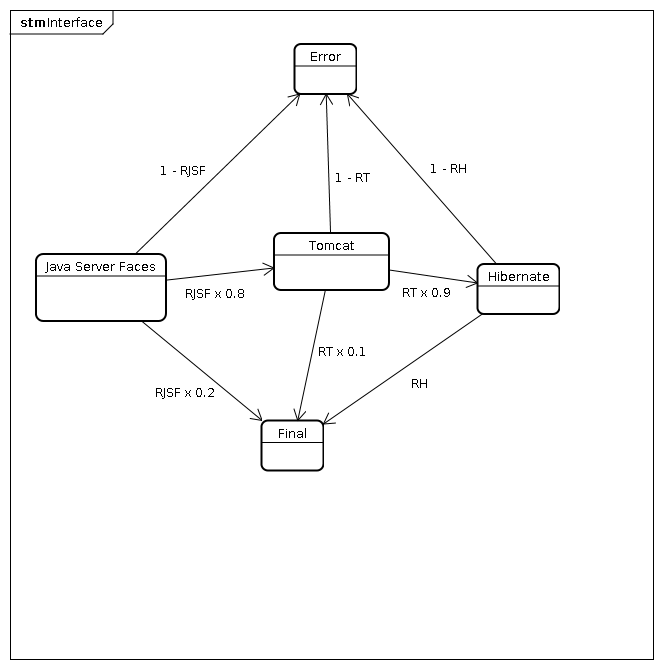
\includegraphics[width=1.0\textwidth]{img/Interface}
\caption{Modelagem analítica da Interface}
\label{fig:anali-inter}
\end{figure}

\begin{figure}[htbp]
\centering
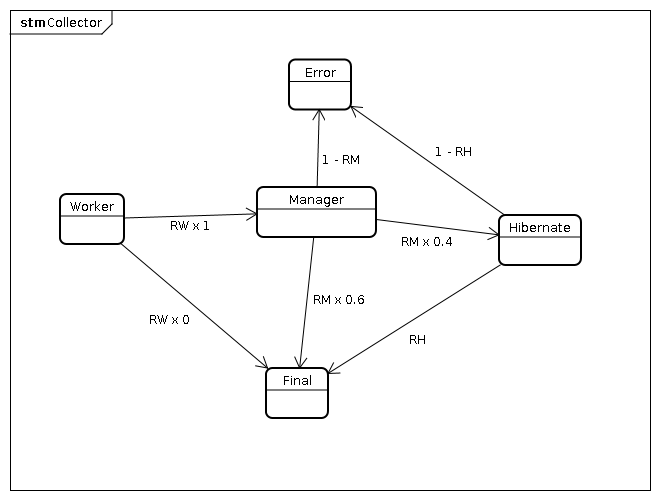
\includegraphics[width=1.0\textwidth]{img/Collector}
\caption{Modelagem analítica do Coletor}
\label{fig:anali-coletor}
\end{figure}

\subsection{Modelo PRISM}
\label{sec:prism}
\begin{verbatim}
dtmc
	const double RT = 0.97; //0.97
	const double RJSF = 0.98; //0.98
	const double RH = 0.83; //0.83

	const double RM = 0.96; //0.96
	const double RW = 1; //1

module Interface
	si : [0..4] init 0;
	
	[] si=0 -> (RT * 0.1) : (si'=3) + (RT * 0.9) : (si'=1) + (1-RT) : (si'=4); //Tomcat
	[] si=1 -> (RJSF * 0.2) : (si'=3) + (RJSF * 0.8) : (si'=2) + (1-RJSF) : (si'=4); //JSF
	[] si=2 -> (RH) : (si'=3) + (1-RH) : (si'=4); //Hibernate
	[] si=3 -> (si'=3); // estado final de sucesso
	[] si=4 -> (si'=4); // estado final de erro
endmodule

module Collector
	sc : [0..4] init 0;
	
	[] sc=0 -> (RW * 0) : (sc'=3) + (RW * 1) : (sc'=1) + (1-RW) : (sc'=4); //Client
	[] sc=1 -> (RM * 0.6) : (sc'=3) + (RM * 0.4) : (sc'=2) + (1-RM) : (sc'=4); //Server
	[] sc=2 -> (RH) : (sc'=3) + (1-RH) : (sc'=4); //Hibernate
	[] sc=3 -> (sc'=3); // estado final de sucesso
	[] sc=4 -> (sc'=4); // estado final de erro
endmodule
\end{verbatim}

\section{Análise quantitativa}
\subsection{Resultados preliminares}
De acordo com a modelagem PRISM, foi possível determinar a
confiabilidade dos módulos de interface e coletor, e do sistema como
um todo.
\begin{description}
\item[Interface] Confiabilidade $C_I = 0.83618656$
\item[Coletor] Confiabilidade $C_C = 0.89472000$
\item[Buzzmap] A confiabilidade do sistema Buzzmap é igual a 1 menos a
chance de pelo menos um dos dos módulos falharem. Como os dois módulos
são independentes, a confiabilidade é $C_B = 1 - (E_C+E_I-E_C*E_I) = 0.748152839$,
    sendo $E_C = 1 - C_C$ a chance de o módulo do coletor falhar, e
    $E_I = 1 - C_I$ a chance de o módulo da interface falhar.
\end{description}

Logo, o sistema Buzzmap fica cerca de 181 horas e 20 minutos por mês
indisponível.


\subsection{Análise de sensibilidade}

\begin{figure}[htbp]
\centering
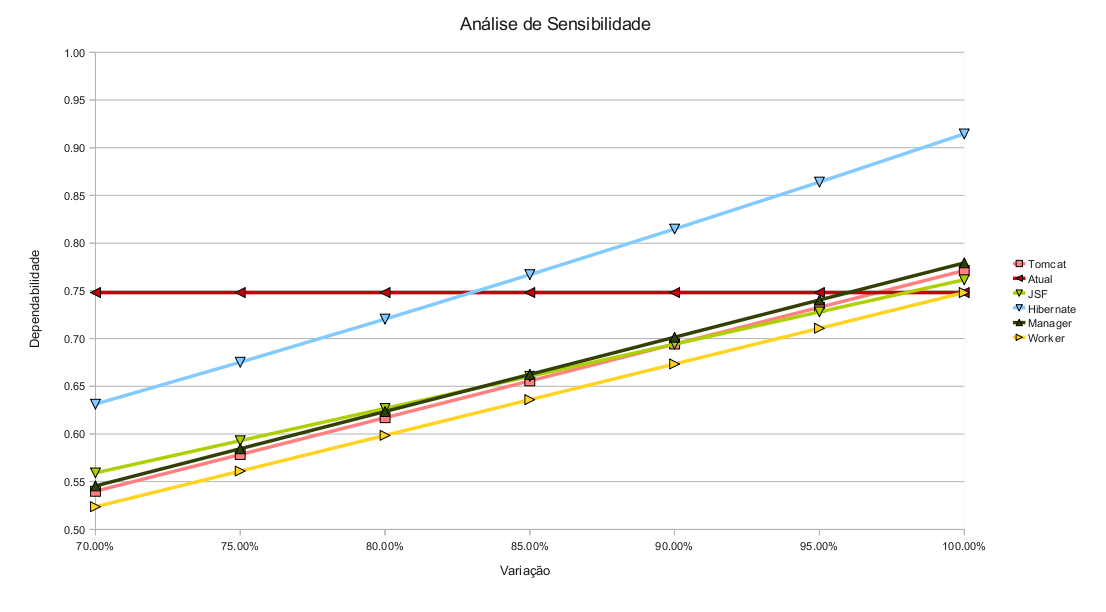
\includegraphics[width=1.0\textwidth]{img/sensibilidade-geral}
\caption{Análise de sensibilidade do sistema Buzzmap}
\label{fig:sensibilidade-geral}
\end{figure}

\begin{figure}[htbp]
\centering
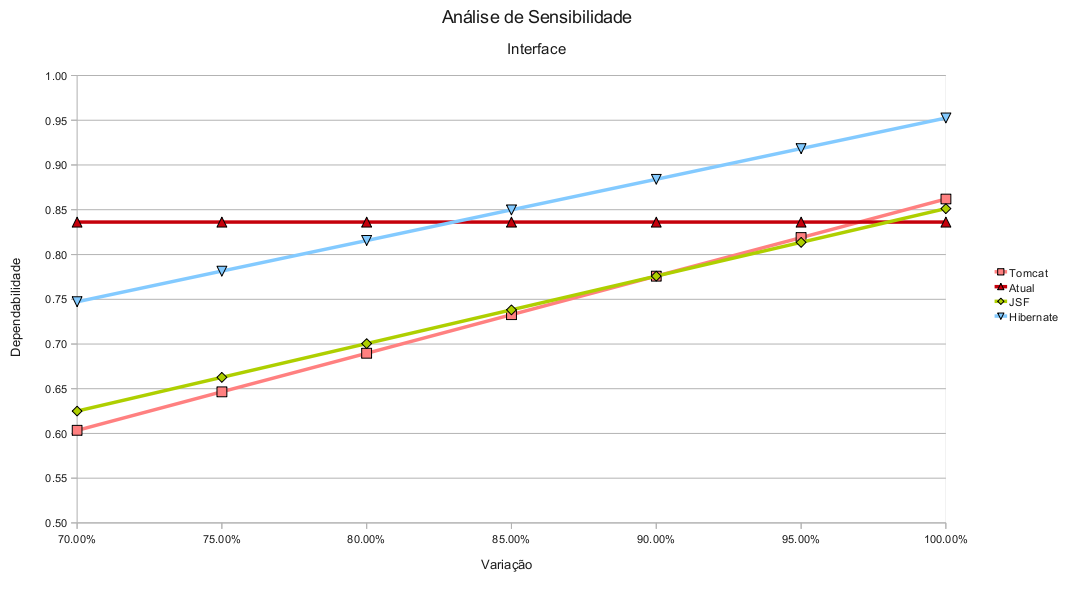
\includegraphics[width=1.0\textwidth]{img/sensibilidade-interface}
\caption{Análise de sensibilidade do módulo de interface}
\label{fig:sensibilidade-interface}
\end{figure}

\begin{figure}[htbp]
\centering
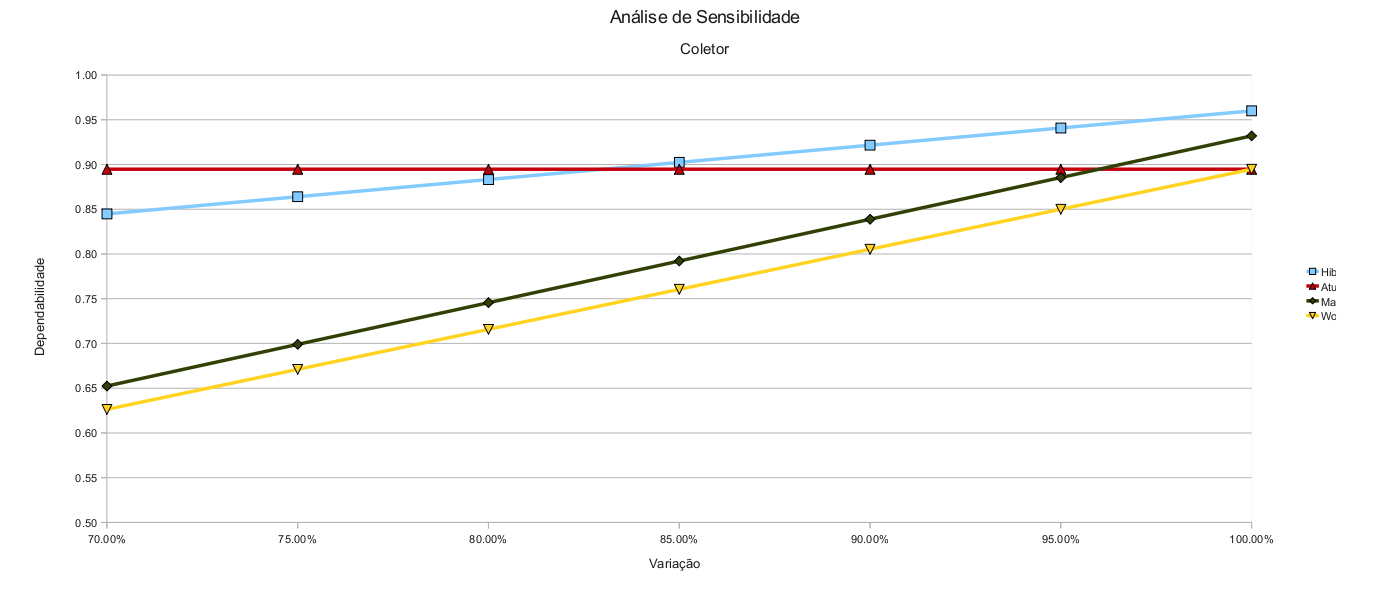
\includegraphics[width=1.0\textwidth]{img/sensibilidade-coletor}
\caption{Análise de sensibilidade do módulo do coletor}
\label{fig:sensibilidade-coletor}
\end{figure}

\section{Avaliação crítica}
Os modelos PRISM foram feitos de forma simplificada devido a cláusulas
de confidencialidade no contrato do sistema Buzzmap. No entanto, ele
dá uma visão alto-nível bastante precisa dos dois principais módulos
do sistema, o coletor e a interface.

Mais ainda, ele reflete claramente o que foi observado informalmente
com o uso do sistema: que ambos os módulos estão bastantes sucetíveis
a falhas, mas que a interface é menos estável que o coletor.

Outro ponto notado com os dados gerados com o PRISM é que o componente
que tem maior influência na confiabilidade dos dois módulos é
justamente o que é comum a ambos, a encapsulação do banco de dados
provida pelo Hibernate. Nos gráficos de análise de sensibilidade, é
possível notar que todos os componente possuem influência linear sobre
a dependabilidade final do sistema, e os componentes mais importantes
são aqueles cujas retas têm maior inclinação e cujo ponto de
interseção com a reta Y é mais alto são as de maior importância, e a
reta representando o Hibernate possui esses dois fatores em escala
maior.

Por isso, é possível concluir que o Hibernate é o componente mais
sensível do sistema Buzzmap. Isso indica que um esforço para aumentar
a confiabilidade deste componente trará maiores ganhos para o sistema
como um todo.
